\documentclass[t]{beamer}
\usepackage[T1]{fontenc}
\usepackage[utf8]{inputenc}  % to be able to type unicode text directly
%\usepackage[french]{babel}   % french typographical conventions
\usepackage{inconsolata}     % for a nicer (e.g. non-courier) tt family font
%\usepackage{amsthm,amsmath}  % fancier mathematics
%\usepackage{array} % to fine-tune tabular spacing
\usepackage{bbm} % for blackboard 1

\usepackage{graphicx}        % to include images
%\usepackage{animate}         % to include animated images
\usepackage{soul}            % for colored strikethrough
%\usepackage{bbding}          % for Checkmark and XSolidBrush
\usepackage{hyperref,url}

\colorlet{darkgreen}{black!50!green}  % used for page numbers
\definecolor{term}{rgb}{.9,.9,.9}     % used for code insets

\setlength{\parindent}{0em}
\setlength{\parskip}{1em}


% coco's macros
\def\R{\mathbf{R}}
\def\F{\mathcal{F}}
\def\x{\mathbf{x}}
\def\y{\mathbf{y}}
\def\u{\mathbf{u}}
\def\Z{\mathbf{Z}}
\def\ud{\mathrm{d}}
\DeclareMathOperator*{\argmin}{arg\,min}
\DeclareMathOperator*{\argmax}{arg\,max}
\newcommand{\reference}[1] {{\scriptsize \color{gray}  #1 }}
\newcommand{\referencep}[1] {{\tiny \color{gray}  #1 }}
\newcommand{\unit}[1] {{\tiny \color{gray}  #1 }}

% disable spacing around verbatim
\usepackage{etoolbox}
\makeatletter\preto{\@verbatim}{\topsep=0pt \partopsep=0pt }\makeatother

% disable headings, set slide numbers in green
\mode<all>\setbeamertemplate{navigation symbols}{}
\defbeamertemplate*{footline}{pagecount}{\leavevmode\hfill\color{darkgreen}
   \insertframenumber{} / \inserttotalframenumber\hspace*{2ex}\vskip0pt}

%% select red color for strikethrough
\makeatletter
\newcommand\SoulColor{%
  \let\set@color\beamerorig@set@color
  \let\reset@color\beamerorig@reset@color}
\makeatother
\newcommand<>{\St}[1]{\only#2{\SoulColor\st{#1}}}
\setstcolor{red}

% make everything monospace
\renewcommand*\familydefault{\ttdefault}

% define a font size tinier than tiny
\makeatletter
\newcommand{\srcsize}{\@setfontsize{\srcsize}{5pt}{5pt}}
\makeatother


\begin{document}

\addtocounter{framenumber}{-1}
\begin{frame}[plain,fragile]
\LARGE\begin{verbatim}





     The Kernel Rank Transform




rafa & enric
cirm 2-7-2025
\end{verbatim}
\end{frame}


\begin{frame}
THE KERNEL RANK TRANSFORM IN ONE SLIDE\\
======================================

{\bf Definition:}
{\color{blue}
	\fbox{
		\color{black}
		\(\displaystyle
		\textsc{KRT}_{{\color{red}\kappa},{\color{red}\sigma}}({\color{blue}u})({\color{blue}x})
		:=
		\int {\color{red}\kappa}({\color{blue}x}-y)\,{\color{red}\sigma}({\color{blue}u(x)}-{\color{blue}u}(y))\,\ud y
		\)
	}
}

\vspace{-0.5em}

{\bf Examples:}

\vspace{-1em}

%MAKE SHELL=/bin/bash

%MAKE all: o/introex5.png o/introex30.png o/introex99.png o/introex190.png
%MAKE o/introex%.png:  i/barbsquare.png; ./krt actualsquare$* $^|qauto -i - $@
\begin{tabular}{cccc}
	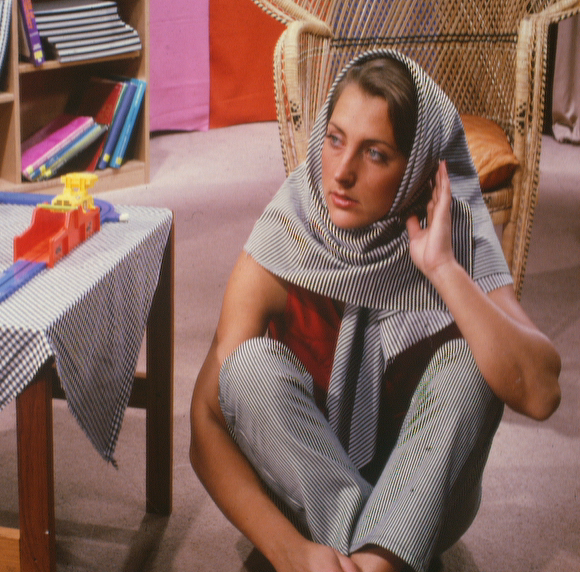
\includegraphics[width=0.2\linewidth]{i/barbara.png}&
	\includegraphics[width=0.2\linewidth]{o/introex5.png}&
	\includegraphics[width=0.2\linewidth]{o/introex30.png}&
	\includegraphics[width=0.2\linewidth]{o/introex190.png}\\
	$u$ &
	$\footnotesize\textsc{KRT}_{{\color{red}g_5},H}(u)$ &
	$\footnotesize\textsc{KRT}_{{\color{red}g_{30}},H}(u)$ &
	$\footnotesize\textsc{KRT}_{{\color{red}g_{200}},H}(u)$
\end{tabular}


%MAKE all: o/fujishadow.png o/fujikrt.png
%MAKE o/fujishadow.png: i/fuji.tif; GETPIXEL=symmetric SHADOWX=-1 SHADOWY=0 plambda $^ 'x,S x,Z 60 * +'|qauto -p 0.1 - $@
%MAKE o/fujikrt.png: i/fuji.tif; ./krt gauss15 -h gap100 $^|plambda '0.5 - 2 *'|downsa v 2|PLEGEND_BGCOLOR=0xaaaaaa palette -1 1 nice -l OVERLAY - $@

%\vspace{-1em}
\vspace{-0.5em}
{\bf Applications:}

	\begin{columns}[b]
		\begin{column}{0.31\textwidth}\scriptsize
$\quad$\\
$\quad$ * noise whitening \\
$\quad$ * dem visualization \\
$\quad$ * image normalization \\
$\quad$ * color balance \\
$\quad$ * cool math\\
%$\quad$ * ...?\\
		\end{column}
		\begin{column}{0.69\textwidth}
			\tiny%\raisebox{5em}{
			\begin{tabular}{cc}
				\includegraphics[width=0.45\linewidth]{o/fujishadow.png}&
				\includegraphics[width=0.45\linewidth]{o/fujikrt.png}\\
				shading(fuji) &
				krt(fuji)
			\end{tabular}
		%}
		\end{column}
	\end{columns}
\end{frame}

%\begin{frame}
%GENEALOGY OF A LEGENDARY POLYCOPIÉ\\
%==================================
%
%\end{frame}

\begin{frame}
OLD VS. NEW\\
===========

\vfill

	\begin{columns}[T]
	\begin{column}{0.5\textwidth}\scriptsize
		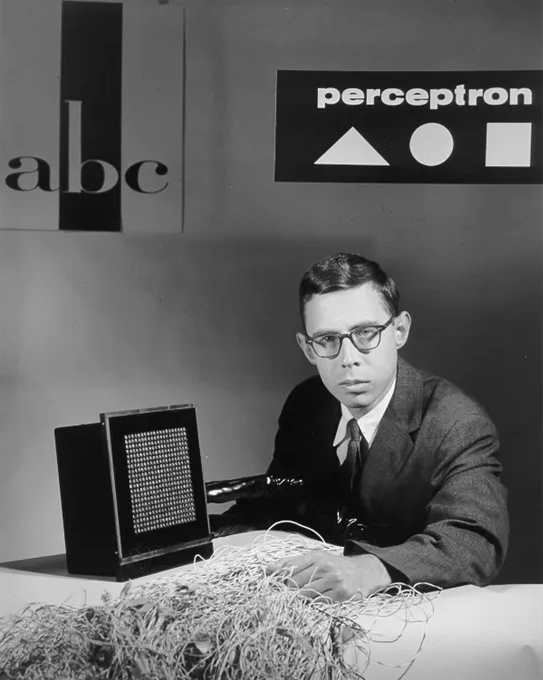
\includegraphics[width=\linewidth]{f/cperceptron.png}
		{\bf F.~Rosenblatt}, {\color{red} 1958}\\
		%\srcsize
		\tiny
		%Two Theorems of Statistical Separability in the Perceptron\\
		3 layer perceptron: projection-association-response
	\end{column}
	\begin{column}[T]{0.5\textwidth}\scriptsize
		\setlength{\parskip}{.6em}
		Newer than the perceptron\\
		-{}-{}-{}-{}-{}-{}-{}-{}-{}-{}-{}-{}-{}-{}-{}-{}-{}-{}-{}-{}-{}-{}-{}-{}-{}

		* Mathematical Morphology (Matheron-Serra, {\color{red}1964})

		* FFT (Cooley-Tuckey, {\color{red}1965})

		* CCD sensors (Boyle-Smith, {\color{red}1969})

		* DCT compression (Ahmed, {\color{red}1972})

		* Anisotropic diffusion\\
		(Perona-Malik, {\color{red}1987})

		* TV denoising (Rudin-Osher-Fatemi, {\color{red}1992})

		* SIFT (Lowe, {\color{red}1999})

		\vfill
		$ $

		Older than the perceptron\\
		-{}-{}-{}-{}-{}-{}-{}-{}-{}-{}-{}-{}-{}-{}-{}-{}-{}-{}-{}-{}-{}-{}-{}-{}-{}

		* PCA (Pearson, {\color{red}1901})

		* Wavelets (Haar,Gabor, {\color{red}1946})
	\end{column}
\end{columns}

\end{frame}

%\begin{frame}
%A COMMENT ABOUT POPULAR SUBJECTS\\
%================================
%$ $%
%
%\vfill
%
%\only<1>{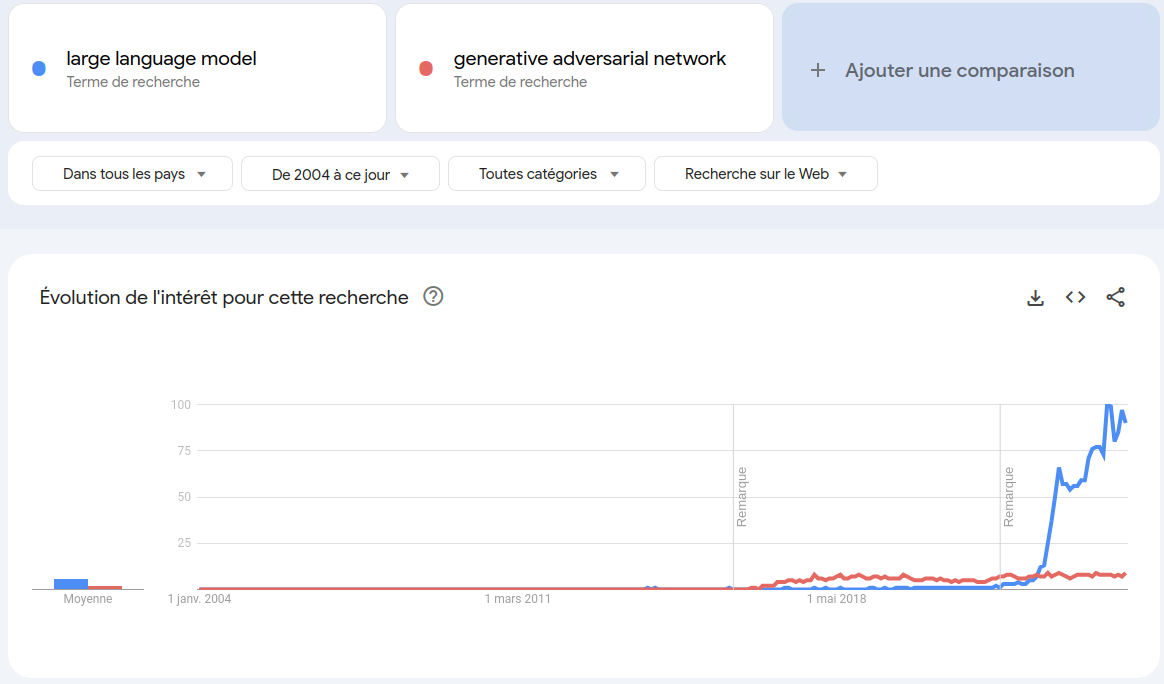
\includegraphics[width=\linewidth]{f/pop_llm_gan.png}}%
%\only<2>{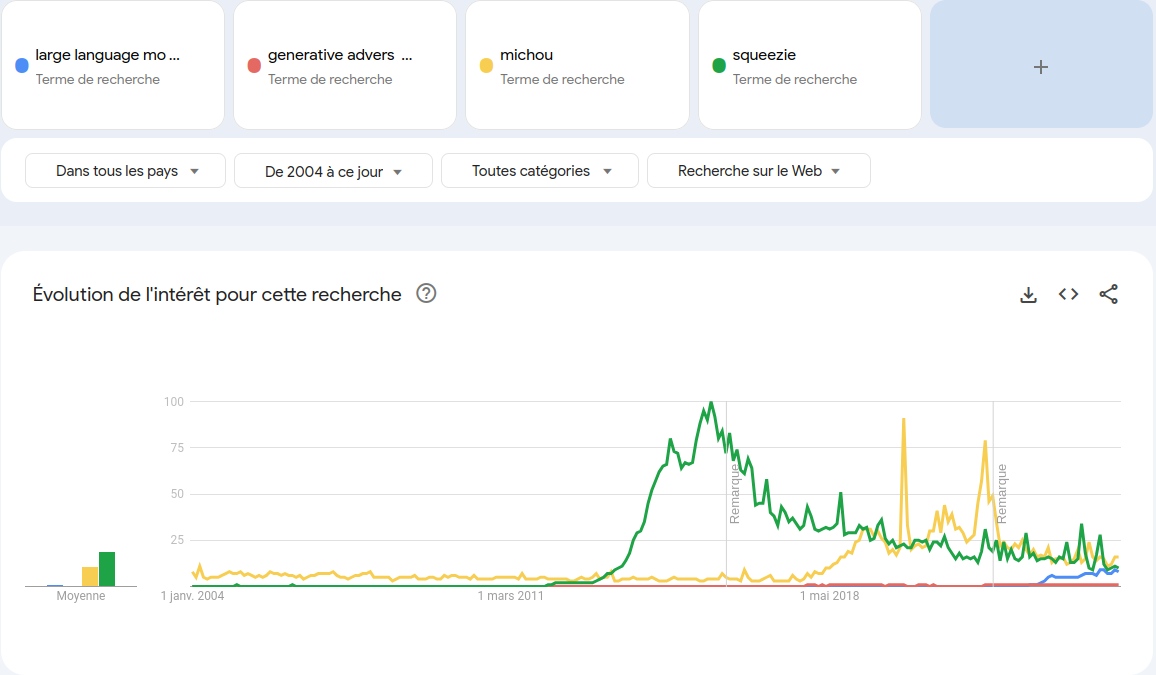
\includegraphics[width=\linewidth]{f/pop_llm_gan2.png}}%
%\only<3>{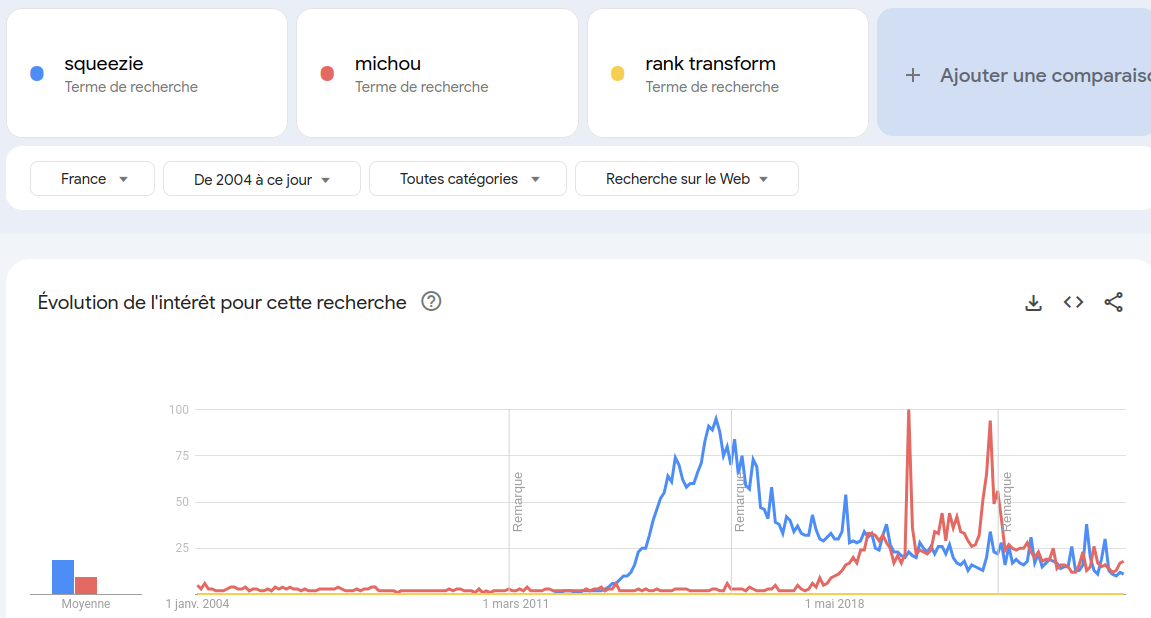
\includegraphics[width=\linewidth]{f/pop_rt.png}}%
%
%Source: {\color{blue}http://trends.google.fr/}
%%GOOGLE TRENDS\\
%%=============
%%
%%	(the joke about popularity being the opposite of originality, with some
%%	related graphs of google trends)
%\end{frame}


\begin{frame}
OUTLINE\\
=======

\vfill

1. Rank Transform\\
$\ \quad${\color{gray}($\approx$ 5min)}

2. Kernel Rank Transform\\
$\ \quad${\color{gray}($\approx$ 15min)}

\vfill

\end{frame}


\begin{frame}[plain,noframenumbering]%

\vfill
\begin{center}
\Huge
--1--\\Rank Transform
\end{center}
\vfill
\small
\centering
{A classical tool in statistics and image processing}
\end{frame}


% 4. rank transform in statistics
\begin{frame}
THE RANK TRANSFORM IN STATISTICS\\
================================

	\begin{tabular}{ll}
		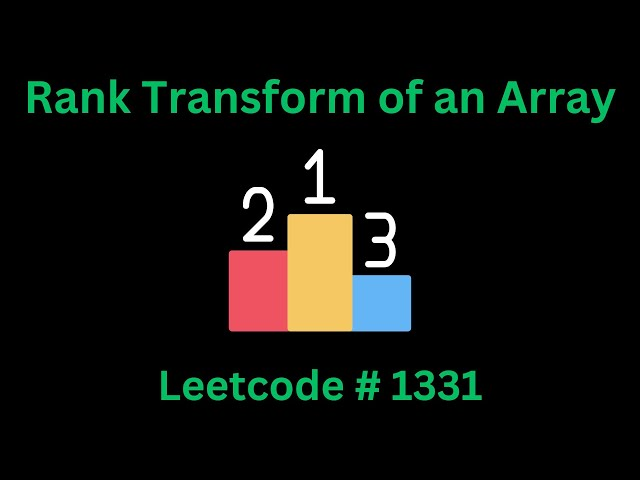
\includegraphics[height=0.3\textheight]{i/indian1.jpg}&
		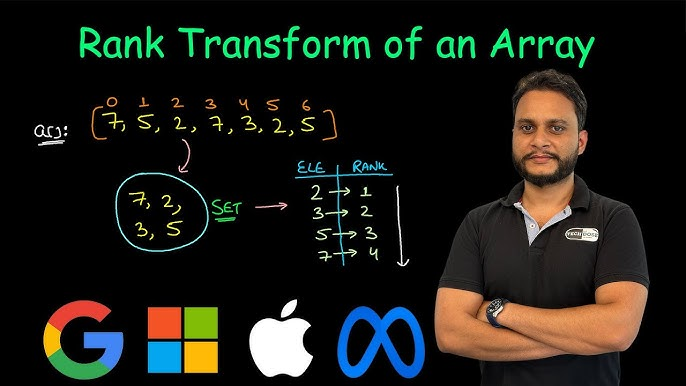
\includegraphics[height=0.3\textheight]{i/indian2.jpg}\\
	\end{tabular}\\
	$ $ Source: {\color{blue}http://www.youtube.com}


	\vfill
	\bigskip
	\vfill

	\pause
	\color{gray}\small

	[0] D.~Quade\\
	{\bf Rank analysis of covariance}\\
	{Journal of the American Statistical Association}, 1967


	[1]  W.~J.~Conover, R.~L.~Iman\\
	{\bf Analysis of covariance using the rank transformation}\\
	{Biometrics}, 1982



\end{frame}



\begin{frame}
RANK TRANSFORM OF AN IMAGE = HISTOGRAM EQUALIZATION\\
===================================================

%MAKE all: o/bgrayhist.png o/bgrayeq.png o/bgrayeqhist.png
%MAKE o/bgrayhist.png:  i/bgra.png; cat $^|ghisto|gnuplot -e 'set term pngcairo size 400,250' ->$@
%MAKE o/bgrayeq.png:  i/bgra.png; cat $^|histeq8|qeasy 0 1 - $@
%MAKE o/bgrayeqhist.png:  i/bgra.png; cat $^|histeq8|blur l 0.6|qeasy 0 1|ghisto|gnuplot -e 'set term pngcairo size 400,250' ->$@

\begin{tabular}{cc}
	$u$ &
	$RT_{\infty}(u) = \textrm{histeq}(u)$\\
	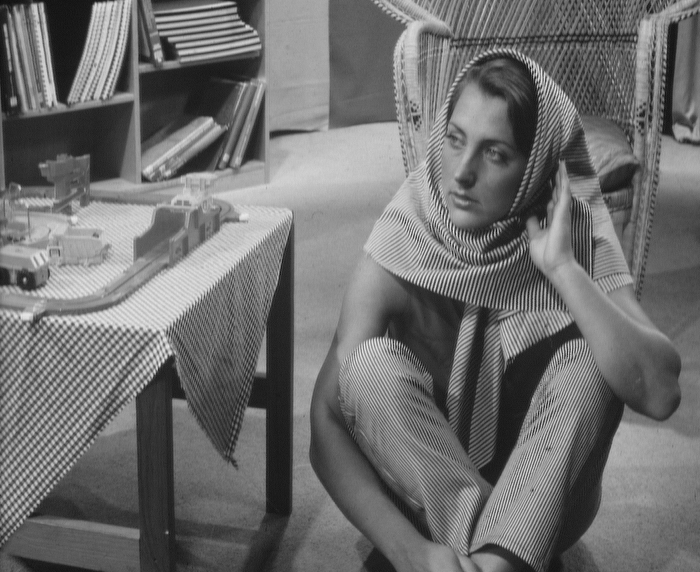
\includegraphics[width=0.47\linewidth]{i/bgra.png}&
	\includegraphics[width=0.47\linewidth]{o/bgrayeq.png}\\
	\includegraphics[width=0.47\linewidth]{o/bgrayhist.png}&
	\includegraphics[width=0.47\linewidth]{o/bgrayeqhist.png}\\
\end{tabular}

\end{frame}



% 5. rank transform in image processing (definitions)
\begin{frame}
THE RANK TRANSFORM IN IMAGE PROCESSING\\
======================================

{\scriptsize\color{gray}
	[2] R.~Zabih, J.~Woodfill\\
	{\bf Non-parametric Local Transforms for Computing Visual Correspondence}\\
	{ECCV, 1994}\\
}
\vspace{-0.5em}
\begin{center}
	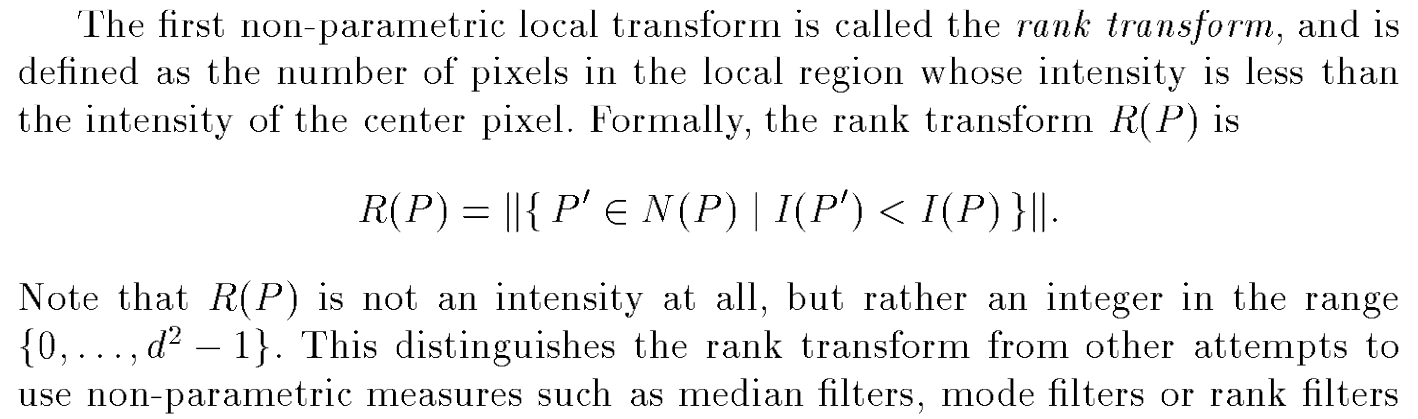
\includegraphics[width=0.7\textwidth]{i/rtdef87.png}
\end{center}

\vfill
\pause

{\scriptsize\color{gray}
	[3] O.~Demetz, D.~Hafner, J.~Weickert\\
	{\bf The Complete Rank Transform}\\
	{BMVC}, 2013\\
}
\vspace{-0.5em}
\begin{center}
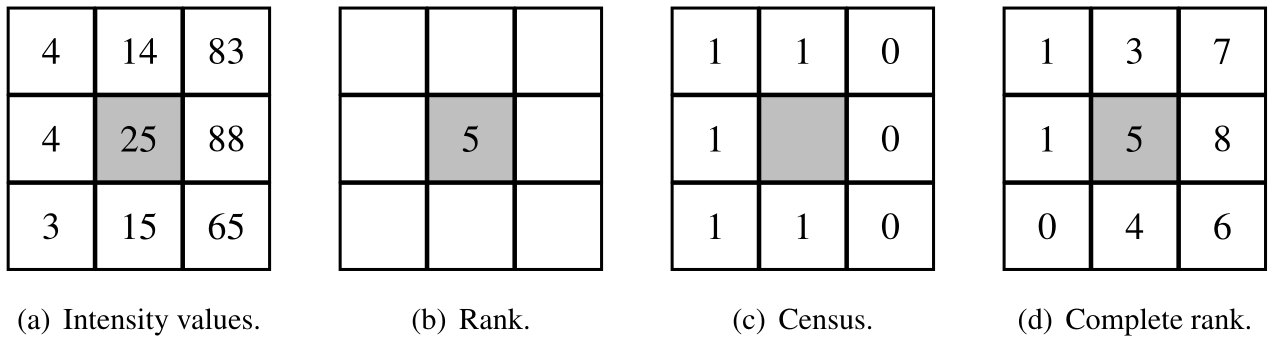
\includegraphics[width=0.7\textwidth]{i/rtfig13.png}
\end{center}



\end{frame}

% (no)6. visualization of the rank transform of various images and window sizes
\begin{frame}
PROPERTIES OF THE RANK TRANSFORM\\
================================

{\bf 1. Contrast-invariance.}
	For increasing~$g:\textbf{R}\to\textbf{R}$:
	\[
		\textsc{RT}_d(u) = \textsc{RT}_d(g\circ u)
	\]

	{\bf 2. Histogram equalization.}
	\[\displaystyle\lim_{d\to\infty}\textsc{RT}_d(u)=\varphi\circ u\]
	where~$\varphi$ is the cumulative distribution function of~$u$.

	{\bf 3. Extrema localization: }\\
	$\qquad\textsc{RT}_d(u)(x)=1$ at local minima, $=d^2$ at local maxima.

	{\bf 4. Visual effect of the parameter }$d$

%MAKE all: o/introex3.png o/introex66.png
\tiny
\begin{tabular}{ccccccc}
	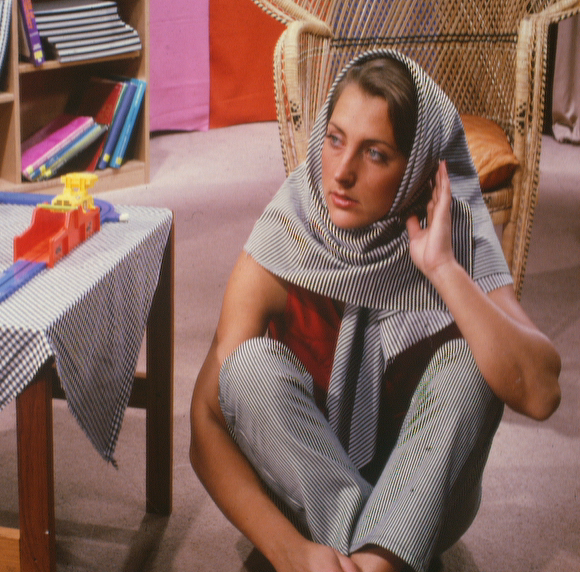
\includegraphics[width=0.1\linewidth]{i/barbara.png}&
	\includegraphics[width=0.1\linewidth]{o/introex3.png}&
	\includegraphics[width=0.1\linewidth]{o/introex5.png}&
	\includegraphics[width=0.1\linewidth]{o/introex30.png}&
	\includegraphics[width=0.1\linewidth]{o/introex66.png}&
	\includegraphics[width=0.1\linewidth]{o/introex99.png}&
	\includegraphics[width=0.1\linewidth]{o/introex190.png}\\
	$u$ &
	$d=3$ &
	$d=5$ &
	$d=30$ &
	$d=66$ &
	$d=99$ &
	$d=200$
\end{tabular}


\end{frame}




\begin{frame}
EFFECT OF THE RANK TRANSFORM ON ELEVATION MAPS\\
==============================================

%MAKE all: o/fuji.png o/fujirg5.png o/fujirg20.png o/fujirg50.png
%MAKE o/fuji.png: i/fuji.tif; palette 0 4000 gray $^ -l OVERLAY $@
%MAKE o/fujirg%.png: i/fuji.tif; ./krt actualsquare$* $^|plambda '$* 2 ^ 1 - * 1 +'|palette 1 $$[$* * $*] gray -l OVERLAY - $@


\begin{tabular}{cc}
	\includegraphics[height=0.38\textheight]{o/fuji.png}&
	\includegraphics[height=0.38\textheight]{o/fujirg5.png}\\
	\includegraphics[height=0.38\textheight]{o/fujirg20.png}&
	\includegraphics[height=0.38\textheight]{o/fujirg50.png}\\
\end{tabular}
\end{frame}

% (no)
% 7. first observation: small window=curvature, large window=histogram equaliz.
\begin{frame}
FIRST MYSTERY: LINK WITH CURVATURE?
===================================

%MAKE all: o/fujik.png  o/fujikd.png
%MAKE all: o/fujir5.png o/fujir5d.png
%MAKE o/fujik.png: i/fuji.tif; plambda $^ 'x,g dup vnorm /'|plambda 'x,d -1 *'|palette -1.3 1.3 nice -l OVERLAY - $@
%MAKE o/fujir5.png: i/fuji.tif; ./krt actualsquare5 $^ |plambda '24 * 1 +'|palette 1 25 nice -l OVERLAY - $@
%MAKE o/fujikd.png: o/fujik.png; plambda TRANS[x=311,y=194,w=200,h=150]:$^ x|ntiply 4 - $@
%MAKE o/fujir5d.png: o/fujir5.png; plambda TRANS[x=311,y=194,w=200,h=150]:$^ x|ntiply 4 - $@

\begin{tabular}{cc}
	\small$\mathrm{div}\left(\frac{\nabla u}{\left\|\nabla u\right\|}\right)$ &
	$\textsc{RT}_5(u)$ \\
	\includegraphics[height=0.38\textheight]{o/fujik.png}&
	\includegraphics[height=0.38\textheight]{o/fujir5.png}\\
	\includegraphics[height=0.38\textheight]{o/fujikd.png}&
	\includegraphics[height=0.38\textheight]{o/fujir5d.png}\\
\end{tabular}


\end{frame}

\begin{frame}[plain,noframenumbering]%

\vfill
\begin{center}
\Huge
--2--\\Kernel Rank Transform
\end{center}
\vfill
\small
\centering
{the subject of our study}
\end{frame}


% 8. integral formulation of the classical rank transform
\begin{frame}
INTEGRAL FORMULATION OF THE RANK TRANSFORM\\
==========================================

\begin{center}
	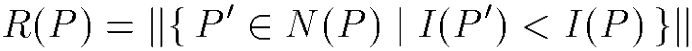
\includegraphics[width=0.7\textwidth]{i/rtdef87c.png}
\end{center}

\begin{center}
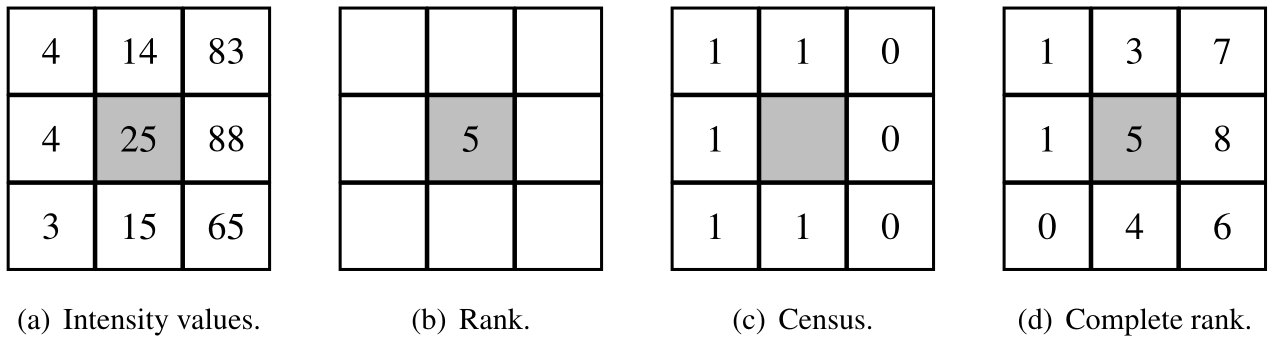
\includegraphics[width=0.7\textwidth]{i/rtfig13.png}
\end{center}

\pause

{\bf Integral formulation:}
%\[
%	R(u)(x) = \int_{N(x)}\textbf{1}_{\left[u < u(x)\right]}(y)\mathrm{d}y
%\]
\[
R({\color{blue}u})({\color{blue}x}) = \int_{N({\color{blue}x})}H({\color{blue}u(x)}-{\color{blue}u}(y))\mathrm{d}y
\qquad
\qquad
\color{gray}H=\textrm{\tiny Heaviside step function}
\]
\pause
\fbox{
\(
	\displaystyle
	\only<3>{R(u)(x) = \int{\color{red}\textbf{1}_{N(0)}}(x-y){\color{red}H}(u(x)-u(y))\mathrm{d}y}
\only<4>{R_{\color{red}\kappa,\sigma}(u)(x) = \int{\color{red}\kappa}(x-y){\color{red}\sigma}(u(x)-u(y))\mathrm{d}y}
\)
}

\end{frame}

% 9. generalization: the KRT
%\begin{frame}
%GENERALIZATION OF THE INTEGRAL FORMULATION\\
%==========================================
%\end{frame}


% 10. formal definition, common gaussian/heaviside cases, generalizes RT
% 11. first formal properties (extreme cases of the parameters)
% 12. visual exploration of the parameters
% 13. first implementation (c code)
% 14. structural properties
% 15. theorem about contrast invariance being a non-differentiable property
% 16. limit for a large kernel
% 17. limit for a vanishingly small kernel, link with curvature (thm)
% 18. ref. alvarez guichard lions evans
% 19. implementation as a convolution in 3D

% 20. particular cases of the KRT, common operators, applications
%   20.1. retinex
%   20.2. dsm/depth image exploration
%   20.3. bilateral filtering
%   20.4. normalizatoin prior to matching (examples w/ cross-correlation scores)
% 21. comparison with other ``whitening'' transforms
%   21.1. laplacian
%   21.2. gradient direction image
%   21.3. integrated gradient direction image
%   21.4. phase image
%   21.5. x-blurred(x)
%   21.6. x-denoised(x)
% 22. summary of particular cases as a 2d table
% 23. choice of implementation depending on parameters
% 24. comparison with perceptron layers / implementation in npu ?

% 25. colophon: source code of the article and the presentation





% 10. formal definition, common gaussian/heaviside cases, generalizes RT
\begin{frame}
DEFINITION OF THE KRT\\
=====================

{\bf Definition.} (Kernel Rank Transform)
For~$u:\textbf{R}^2\to\textbf{R}$,
\[
	R_{\color{red}\kappa,\sigma}(u)(x) = \int{\color{red}\kappa}(x-y){\color{red}\sigma}(u(x)-u(y))\mathrm{d}y
\]
where
\[
	{\color{red}\kappa}:\textbf{R}^2\to\textbf{R}\qquad\qquad\textrm{``the kernel''}
\]
\[
	{\color{red}\sigma}:\textbf{R}\to\textbf{R}\ \ \qquad\qquad\textrm{``the gap''}
\]

\pause

{\bf Typical kernels:}\\
$g_s=$ gaussian of size~$s$, $N_d=$ square of side~$d$

{\bf Typical gaps:} $H=$ Heaviside step function,\\
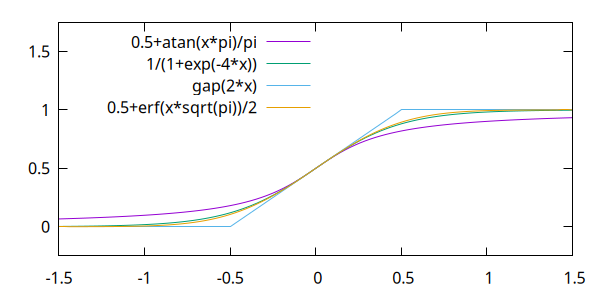
\includegraphics[height=0.25\textheight]{f/plot_heavisides.png}
%SCRIPT gnuplot > f/plot_heavisides.png <<EOF
%SCRIPT set term pngcairo size 600,300
%SCRIPT set key top left
%SCRIPT gap(x)=x>1?1:(x<-1?0:(0.5*(x+1)))
%SCRIPT plot [-1.5:1.5] [-0.25:1.75] 0.5+atan(x*pi)/pi,1/(1+exp(-4*x)),gap(2*x),0.5+erf(x*sqrt(pi))/2
%SCRIPT EOF


\end{frame}

\begin{frame}
DISCRETE KRT\\
============

\[
	KRT_{\kappa,\,\sigma}(u)(x) = \sum_{y\in\textbf{Z}^2}\kappa(x-y)\sigma(u(x)-u(y))
\]

Naïve implementation $O(N^2)$~:

Fancier implementaiton $O(QN\log N)$~:

\end{frame}


% 11. first formal properties (extreme cases of the parameters)
\begin{frame}
GENERAL PROPERTIES OF THE KRT\\
=============================

{\bf P1.} If~$u$ is constant then~$R_{\kappa,\sigma}(u)=\sigma(0)\int\kappa$

{\bf P2.} Scaling and shifting:
$R_{\kappa,\,{\color{red}a}\sigma+{\color{red}b}}={\color{red}a}\,R_{\kappa,\sigma}+{\color{red}b}\int\kappa$.

{\bf P3.} Symmetry: $\R_{\kappa,\sigma}({\color{red}-}u)={\color{red}-}R_{\kappa,\sigma}(u)\quad$ (if~$\sigma$ is odd)

{\bf P5.} Affine covariance:
\( R_{\kappa,\sigma}\left(u\circ{\color{red}\varphi}\right) =
R_{{\color{red}\tilde\kappa},\sigma}\left(u\right)\circ\color{red}\varphi\)
		where~$\varphi(x)=Ax+b$ and $\tilde\kappa=\frac1{|A|}\kappa\circ A^{-1}$.

		{\bf P6.} Locality: $R_{\kappa,\sigma}(u)(x)$ only depends on~$u|_{\{x+y:y\in\mathrm{supp}(\kappa)\}}$


\end{frame}

\begin{frame}
PROPERTIES FOR THE HEAVISIDE CASE\\
=================================

{\bf H1.} Contrast-invariance:
for any increasing~$\color{red}g$
$$R_{\kappa,H}({\color{red}g}\circ u)=R_{\kappa,H}(u)$$
\pause

{\bf H2.} For~$x=\mathrm{argmax}(u)$, $R_{\kappa,H}(u)(x)=\int\kappa$.

{\bf H3.} For~$x=\mathrm{argmin}(u)$, $R_{\kappa,H}(u)(x)=0$.
\end{frame}


% noise whitening experiment
\begin{frame}
NOISE UNIFORMIZATION BY KRT\\
===========================

%MAKE: all: o/wramp.png o/wramphist.png o/wramptex.png
%MAKE: all: o/wrampk7.png o/wrampk7hist.png o/wrampk7tex.png
%MAKE: o/wramp.png: o/wramp.npy ; qauto -p 1 $^ $@
%MAKE: o/wramp.npy: ; plambda zero:400x300 'randg :i *' -o $@
%MAKE: o/wramphist.png: o/wramp.npy ; plambda $^ round|ghisto|gnuplot -e 'set term pngcairo size 400,300' ->$@
%MAKE: o/wrampk7.png: o/wrampk7.npy ; qeasy 0 1 $^ $@
%MAKE: o/wrampk7.npy: o/wramp.npy ; krt actualsquare7 $^ $@
%MAKE: o/wrampk7hist.png: o/wrampk7.npy ; plambda $^ '48 * round'|ghisto|gnuplot -e 'set term pngcairo size 400,300' ->$@
%MAKE: o/wramptex.png: o/wramp.npy ; autocorr $^|croparound 200 150 50 37|sauto -s 3e8|ntiply 8 - $@
%MAKE: o/wrampk7tex.png: o/wrampk7.npy ; autocorr $^|croparound 200 150 50 37|sauto -s 300|ntiply 8 - $@

%MAKE: all: o/wrampg4.png o/wrampg4hist.png o/wrampg4tex.png
%MAKE: o/wrampg4.png: o/wrampg4.npy ; qeasy 0 1 $^ $@
%MAKE: o/wrampg4.npy: o/wramp.npy ; krt gauss4 $^ $@
%MAKE: o/wrampg4hist.png: o/wrampg4.npy ; plambda $^ '100 * round'|ghisto|gnuplot -e 'set term pngcairo size 400,300' ->$@
%MAKE: o/wrampg4tex.png: o/wrampg4.npy ; autocorr $^|croparound 200 150 50 37|sauto -s 300|ntiply 8 - $@

\begin{tabular}{lll}
	\includegraphics[width=0.3\linewidth]{o/wramp.png} &
	\includegraphics[width=0.3\linewidth]{o/wramphist.png} &
	\includegraphics[width=0.3\linewidth]{o/wramptex.png} \\
	$u(x,y)=x\mathcal{W}(x,y)$ &
	$\mathrm{hist}(u)$ &
	$\mathrm{autocorr}(u)$\\
	&&\\
	\only<1>{%
	\includegraphics[width=0.3\linewidth]{o/wrampk7.png} &
	\includegraphics[width=0.3\linewidth]{o/wrampk7hist.png} &
	\includegraphics[width=0.3\linewidth]{o/wrampk7tex.png} \\
	$\textsc{KRT}_{\color{red}7}(u)$ &
	$\mathrm{hist}(\textsc{KRT}_{\color{red}7}(u))$ &
	$\mathrm{autocorr}(\textsc{KRT}_{\color{red}7}(u))$
	}\only<2>{%
	\includegraphics[width=0.3\linewidth]{o/wrampg4.png} &
	\includegraphics[width=0.3\linewidth]{o/wrampg4hist.png} &
	\includegraphics[width=0.3\linewidth]{o/wrampg4tex.png} \\
	$\textsc{KRT}_{\color{red}G_4}(u)$ &
	$\mathrm{hist}(\textsc{KRT}_{\color{red}G_4}(u))$ &
	$\mathrm{autocorr}(\textsc{KRT}_{\color{red}G_4}(u))$
	}
\end{tabular}

	{\color{red}
	\fbox{
	\footnotesize
	{\bf Thm.} If $\color{black}X=\textsc{KRT}_{\kappa}(\mathcal{W})$
	then $\color{black}X_p\sim\mathcal{U}(0,1)$
	and  $\color{black}\mathrm{cov}(X_p,X_q)\approx-\kappa(p-q)$
	}
	}

\end{frame}

% 


% 12. visual exploration of the parameters
\begin{frame}
EXPLORATION OF THE PARAMETERS\\
=============================

%MAKE: all: o/starsr5.png o/starsr50.png o/bstars.png o/bstarsr5.png o/bstarsr50.png
%MAKE: o/bstars.npy: i/stars.png; blur l 0.61 $^ $@
%MAKE: o/bstars.png: o/bstars.npy; qauto -p 0 $^ $@
%MAKE: o/starsr%.png: i/stars.png; ./krt gauss$* $^|qauto -p 0 - $@
%MAKE: o/bstarsr%.png: o/bstars.npy; ./krt gauss$* $^|qauto -p 0 - $@
%MAKE: o/bstarsgr%.png: o/bstars.npy; ./krt -h gap0.01 gauss$* $^|qauto -p 0 - $@
%MAKE: all: o/bstarsgr5.png o/bstarsgr50.png

\scriptsize
\begin{tabular}{ccc}
	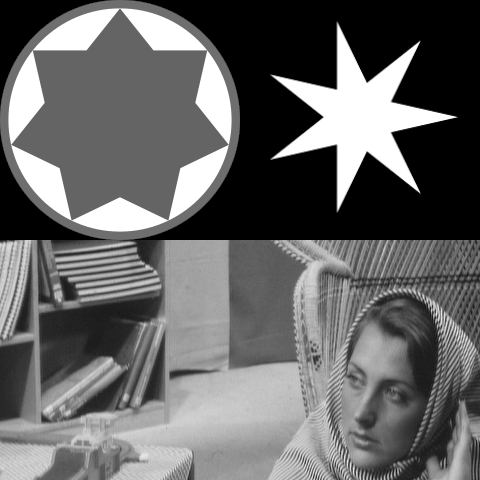
\includegraphics[width=0.3\linewidth]{i/stars.png}&
	\includegraphics[width=0.3\linewidth]{o/starsr5.png}&
	\includegraphics[width=0.3\linewidth]{o/starsr50.png}\\
	$u$ &
	$R_{g_5,H}(u)$ &
	$R_{g_{50},H}(u)$ \\
	&&\\
	\pause
	\only<2>{
	\includegraphics[width=0.3\linewidth]{o/bstars.png}&
	\includegraphics[width=0.3\linewidth]{o/bstarsr5.png}&
	\includegraphics[width=0.3\linewidth]{o/bstarsr50.png}\\
	$g_\epsilon*u$ &
	$R_{g_5,\color{red}H}(g_\epsilon*u)$ &
	$R_{g_{50},\color{red}H}(g_\epsilon*u)$ \\
}\only<3>{
	\includegraphics[width=0.3\linewidth]{o/bstars.png}&
	\includegraphics[width=0.3\linewidth]{o/bstarsgr5.png}&
	\includegraphics[width=0.3\linewidth]{o/bstarsgr50.png}\\
	$g_\epsilon*u$ &
	$R_{g_5,\color{red}\sigma_{0.001}}(g_\epsilon*u)$ &
	$R_{g_{50},\color{red}\sigma_{0.001}}(g_\epsilon*u)$ \\
}
\end{tabular}
\end{frame}

\begin{frame}
CONTRAST-INVARIANCE VS. DIFFERENTIABILITY\\
=========================================

{\bf Definition.}
An image operator~$T:u\mapsto T(u)$ is {\color{blue}contrast-invariant}
if~$T(g\circ u)=T(u)$ for any increasing~$g$.

{\bf Proposition 1.}
If~$T$ is continuous and contrast-invariant then it is trivial: $T(u)=T(0)$ for
any~$u$).

\pause

{\color{gray}
Proof: the path~$\lambda\mapsto\lambda u$ links any image $u$ to~$0$.
}

\pause
\vfill
\color{red}
\fbox{
\fbox{
Contrast-invariance is a non-differentiable property
}}
\vfill

\end{frame}




\begin{frame}
EXTREME CASES\\
=============

{\color{blue}
	\fbox{
		\color{black}
		\(\displaystyle
		R_{{\color{red}\kappa},{\color{red}\sigma}}({\color{blue}u})({\color{blue}x})
		:=
		\int {\color{red}\kappa}({\color{blue}x}-y)\,{\color{red}\sigma}({\color{blue}u(x)}-{\color{blue}u}(y))\,\ud y
		\)
	}
}

When~$\sigma\to id$:
\[
	R_{\kappa, id}(u) = u - k*u
\]
{\color{gray}This is a good approximation of~$-\Delta u$ for small~$\kappa$.}

\pause
{\bf Proposition 2.}
Let $\sigma$ be a smooth gap and~$\kappa$ be a normalized kernel.
Set~$\kappa_h(x)=\kappa(x/h)/h^2$, then
\[
	R_{\kappa_{\color{red}h},\sigma}(u)(x)
	=
	s(0)
	-\frac{s'(0)}2\Delta u(x){\color{red}h}^2
	+O({\color{red}h}^3)
\]

\pause
\color{red}
\fbox{\fbox{
		$\displaystyle\lim_{t\to0}R_{g_t,\color{blue}\sigma}(u)= -\Delta u$
}}
\pause
\fbox{\fbox{
		$\displaystyle\lim_{t\to0}R_{g_t,\color{blue}H}(u)= \color{black}???$
}}

\end{frame}




\begin{frame}
WHY DO WE FIND THE CURVATURE\\
============================

\only<1>{
\includegraphics[width=\textwidth]{f/figure1.png}
}
\only<2>{
	\includegraphics[width=0.6\textwidth]{f/figure1.png}

	\vfill

$R_{g_\epsilon,H}(u)({\color{red}b})=\frac12$

$R_{g_\epsilon,H}(u)({\color{red}a})\to\frac12$

$R_{g_\epsilon,H}(u)({\color{red}c})\to\frac12$

$R_{g_\epsilon,H}(u)({\color{red}d})\to\frac{\mathrm{angle}}{2\pi}$
}
\only<3>{\includegraphics[height=0.8\textheight]{f/pcurv.png}}
\only<4>{\includegraphics[height=0.5\textheight]{f/pcurv.png}

	\vfill

	{\bf Proposition 3.}
	If the level curve of~$u$ through~$x$ is smooth;
set~$\kappa_h(x)=\kappa(x/h)/h^2$, then
\[
	R_{\kappa_{\color{red}h},H}(u)(x)
	=
	\frac12
	+\frac1{4\pi}\mathrm{curv}(u)(x){\color{red}h}+O({\color{red}h}^2)
\]
with~$\mathrm{curv}(u)=\mathrm{div}\left(\frac{\nabla u}{\left\|\nabla u\right\|}\right)$
}


\end{frame}

\begin{frame}
MYSTERY EXPLAINED!\\
==================


\begin{tabular}{cc}
	\small$\mathrm{div}\left(\frac{\nabla u}{\left\|\nabla u\right\|}\right)$ &
	$\textsc{R}_{g_3,H}(u)$ \\
	\includegraphics[height=0.38\textheight]{o/fujik.png}&
	\includegraphics[height=0.38\textheight]{o/fujir5.png}\\
	\includegraphics[height=0.38\textheight]{o/fujikd.png}&
	\includegraphics[height=0.38\textheight]{o/fujir5d.png}\\
\end{tabular}

\end{frame}


\begin{frame}
TABLE OF INFINITESIMAL GENERATORS
=================================

\end{frame}




\begin{frame}
RELATIONSHIP WITH BILATERAL FILTERS
===================================

\end{frame}


\begin{frame}
APPLICATION: NOISE UNIFORMISATION\\
=================================

(example with synthetic image "randg :i *")

\end{frame}


\begin{frame}
APPLICATION: NOISE UNIFORMISATION\\
=================================

(example "calanques")

\end{frame}



\begin{frame}
APPLICATION: SIMULATION OF PERCEPTION (retinex)\\
===============================================

\vfill

\only<1>{
\begin{tabular}{cc}
	\includegraphics[width=0.43\linewidth]{f/adelson.png} &
	\includegraphics[width=0.43\linewidth]{f/adelson_l25_gap200.png} \\
\end{tabular}
}\only<2>{
	%\includegraphics[height=0.83\textheight]{f/machs.png}\\
	mach bands
}

\vfill

\end{frame}


\begin{frame}
APPLICATION: CLEANER CROSS-CORRELATIONS\\
=======================================

%\begin{tabular}{cc}
%	\includegraphics[width=0.43\linewidth]{f/i12345.png} &
%	\includegraphics[width=0.43\linewidth]{f/t12345.jpg} \\
%	\includegraphics[width=0.43\linewidth]{f/plaincorr_i_t.png} &
%	\includegraphics[width=0.43\linewidth]{f/croscorr_i_t.png} \\
%\end{tabular}

\end{frame}


\begin{frame}
PERSPECTIVE: A NEW KIND OF PERCEPTRON?\\
======================================

Typical perceptron layer:
\[
	u'_i \gets {\color{red}\sigma}\left(\sum_j k_{ij}u_j\right)
\]

\pause

Contrast-invariant perceptron:
\[
	u'_i \gets \sum_j k_{ij}{\color{red}\sigma}(u_i-u_j)
\]

\end{frame}



\begin{frame}
COLOPHON\\
========


\end{frame}



\end{document}

% 13. first implementation (c code)
\begin{frame}
IMPLEMENTATION\\
==============

	\includegraphics[width=\textwidth]{i/krtcode.png}

\end{frame}

% 14. structural properties
\begin{frame}
STRUCTURAL PROPERTIES\\
=====================
\end{frame}

% 15. theorem about contrast invariance being a non-differentiable property
\begin{frame}
CONTRAST INVARIANCE\\
===================
\end{frame}

% 16. limit for a large kernel
\begin{frame}
LIMIT FOR LARGE KERNELS\\
=======================
\end{frame}

% 17. limit for a vanishingly small kernel, link with curvature (thm)
\begin{frame}
LIMIT FOR SMALL KERNELS\\
=======================

	(maybe separate the cases into two or three slides)
\end{frame}

% 18. ref. alvarez guichard lions evans
\begin{frame}
	(ref. alvarez guichard lions evans)
\end{frame}

% 19. implementation as a convolution in 3D
\begin{frame}
INTERPRETATION IN 3D\\
====================
\end{frame}


% 20. particular cases of the KRT, common operators, applications
\begin{frame}
PARTICULAR CASES OF THE KRT\\
===========================
\end{frame}

%   20.1. retinex
\begin{frame}
	retinex\\
=============
\end{frame}

%   20.2. dsm/depth image exploration
\begin{frame}
	dsm/depth image exploration\\
=============
\end{frame}

%   20.3. bilateral filtering
\begin{frame}
	bilateral filtering\\
=============
\end{frame}

%   20.4. normalizatoin prior to matching (examples w/ cross-correlation scores)
\begin{frame}
	normalization prior to matching\\
=============
\end{frame}

% 21. comparison with other ``whitening'' transforms
\begin{frame}
COMPARISON WITH OTHER ``WHITENING'' TRANSFORMS\\
==============================================
\end{frame}

%%   21.1. laplacian
%\begin{frame}
%=============
%\end{frame}
%
%%   21.2. gradient direction image
%\begin{frame}
%=============
%\end{frame}
%
%%   21.3. integrated gradient direction image
%\begin{frame}
%=============
%\end{frame}
%
%%   21.4. phase image
%\begin{frame}
%=============
%\end{frame}
%
%%   21.5. x-blurred(x)
%\begin{frame}
%=============
%\end{frame}
%
%%   21.6. x-denoised(x)
%\begin{frame}
%=============
%\end{frame}

% 22. summary of particular cases as a 2d table
\begin{frame}
PARTICULAR CASES OF THE KRT\\
===========================
\end{frame}

% 23. choice of implementation depending on parameters
\begin{frame}
CHOICE OF IMPLEMENTATION DEPENDING ON THE PARAMETERS\\
====================================================
\end{frame}

% 24. comparison with perceptron layers / implementation in npu ?
\begin{frame}
COMPARISON WITH A PERCEPTRON LAYER\\
==================================
\end{frame}


% 25. colophon: source code of the article and the presentation
\begin{frame}
COLOPHON\\
========
\end{frame}






\end{document}


% vim:sw=2 ts=2 :
